%% Copernicus Publications Manuscript Preparation Template for LaTeX Submissions
%% ---------------------------------
%% This template should be used for copernicus.cls
%% The class file and some style files are bundled in the Copernicus Latex Package, which can be downloaded from the different journal webpages.
%% For further assistance please contact Copernicus Publications at: production@copernicus.org
%% https://publications.copernicus.org/for_authors/manuscript_preparation.html

%% copernicus_rticles_template (flag for rticles template detection - do not remove!)

%% Please use the following documentclass and journal abbreviations for discussion papers and final revised papers.

%% 2-column papers and discussion papers
\documentclass[gc, manuscript]{copernicus}



%% Journal abbreviations (please use the same for discussion papers and final revised papers)


% Advances in Geosciences (adgeo)
% Advances in Radio Science (ars)
% Advances in Science and Research (asr)
% Advances in Statistical Climatology, Meteorology and Oceanography (ascmo)
% Annales Geophysicae (angeo)
% Archives Animal Breeding (aab)
% ASTRA Proceedings (ap)
% Atmospheric Chemistry and Physics (acp)
% Atmospheric Measurement Techniques (amt)
% Biogeosciences (bg)
% Climate of the Past (cp)
% DEUQUA Special Publications (deuquasp)
% Drinking Water Engineering and Science (dwes)
% Earth Surface Dynamics (esurf)
% Earth System Dynamics (esd)
% Earth System Science Data (essd)
% E&G Quaternary Science Journal (egqsj)
% Fossil Record (fr)
% Geochronology (gchron)
% Geographica Helvetica (gh)
% Geoscience Communication (gc)
% Geoscientific Instrumentation, Methods and Data Systems (gi)
% Geoscientific Model Development (gmd)
% History of Geo- and Space Sciences (hgss)
% Hydrology and Earth System Sciences (hess)
% Journal of Micropalaeontology (jm)
% Journal of Sensors and Sensor Systems (jsss)
% Mechanical Sciences (ms)
% Natural Hazards and Earth System Sciences (nhess)
% Nonlinear Processes in Geophysics (npg)
% Ocean Science (os)
% Primate Biology (pb)
% Proceedings of the International Association of Hydrological Sciences (piahs)
% Scientific Drilling (sd)
% SOIL (soil)
% Solid Earth (se)
% The Cryosphere (tc)
% Web Ecology (we)
% Wind Energy Science (wes)


%% \usepackage commands included in the copernicus.cls:
%\usepackage[german, english]{babel}
%\usepackage{tabularx}
%\usepackage{cancel}
%\usepackage{multirow}
%\usepackage{supertabular}
%\usepackage{algorithmic}
%\usepackage{algorithm}
%\usepackage{amsthm}
%\usepackage{float}
%\usepackage{subfig}
%\usepackage{rotating}


% The "Technical instructions for LaTex" by Copernicus require _not_ to insert any additional packages.
%
\usepackage{algorithmic}
\usepackage{algorithm}


\begin{document}

\title{GeoChronR}


\Author[1]{Nicholas}{McKay}
\Author[2]{Julien}{Emile-Geay}
\Author[2]{Deborah}{Khider}


\affil[1]{School of Earth and Sustainability, Northern Arizona University,
Flagstaff, AZ 86011}
\affil[2]{University of Southern California, Los Angeles, CA}

%% The [] brackets identify the author with the corresponding affiliation. 1, 2, 3, etc. should be inserted.



\runningtitle{GeoChronR title}

\runningauthor{McKay et al.}


\correspondence{Nicholas\ McKay\ (Nicholas.McKay@nau.edu)}



\received{}
\pubdiscuss{} %% only important for two-stage journals
\revised{}
\accepted{}
\published{}

%% These dates will be inserted by Copernicus Publications during the typesetting process.


\firstpage{1}

\maketitle


\begin{abstract}
The abstract goes here. It can also be on \emph{multiple lines}.
\end{abstract}


\copyrightstatement{The author's copyright for this publication is transferred to
institution/company.}


\introduction

\subsection{Background}

Review the need for, and examples of age uncertain analysis in the
literature.

\subsection{Motivation}

Why we built geoChronR

\subsection{Outline of manuscript}

Should we include this section?

\section{Workflow}

\subsection{Installation and setup}

\subsection{File input/output}

\subsection{Integrated geochronology uncertainty quantification
software}

\subsubsection{Bacon}

\subsubsection{BChron}

\subsubsection{Oxcal}

\subsubsection{Banded Age Models (BAM)}

\subsection{Age-uncertain analytical tools}

Intro on analytical approach, using ensembles\ldots{}.

\subsubsection{Correlation}

\subsubsection{Regression}

\subsubsection{Principle Components Analysis}

\subsubsection{Spectral Analysis}

\subsection{Visualization}

\subsubsection{Timeseries}

\subsubsection{Geospatial}

\subsubsection{Power spectra}

\section{Use cases}

What's the point of these use cases.

\subsection{Creating an age ensemble}

A common first task when using geoChronR is to create an age ensemble,
either because the user is developing a new record, or because the age
ensemble data for the record they are interested is unavailable. As
described in section X.Y workflows for four published age quantification
programs are integrated into geoChronR. Bacon \citep{bacon}, BChron
\citep{parnell2008flexible}, and OxCal \citep{ramsey2008deposition} are
Bayesian age-deposition models that estimate posteriors on age-depth
relationships with different assumptions and methodologies. BAM
\citep{BAM} was designed to probabilistically simulate counting
uncertainty in banded archives, such as corals, ice cores, or varved
sediments, but can also be used to simulate age uncertainty for any
record, and is useful when the data or metadata required to calculate an
age-depth model are unavailable. All four methods are mostly simply used
in geoChronR with a LiPD file that contains the chronological
measurements, and the functions \texttt{runBacon(L)},
\texttt{runBchron(L)}, \texttt{runOxcal(L)} and \texttt{runBam(L)}.
These functions take LiPD objects as inputs, and return updated LiPD
objects that include age-ensemble data generated by the respective
software packages. Typically, additional parameters are needed for to
optimally run the algorithms. When these parameters are not included,
geoChronR will run in interactive mode, asking the user which variables
and parameters they would like to model. These parameter choices are
printed to the screen during while the program runs, or are available
later with the function \texttt{getLastVarString()}. By specifying these
parameters, age model creation can be scripted and will run in
non-interactive mode. In this use case, we'll use geoChronR and BChron
\citep{parnell2008flexible} to calculate an age ensemble for the Hulu
Cave \(\delta^{18}\)O speleothem record \citep{hulu2001}, and BAM
\citep{BAM} to simulate age uncertainties for the GISP2 ice core
\(\delta^{18}\)O dataset \citep{alley}. The \texttt{plotChronEns(hulu)}
function will plot an age-depth model and uncertainties derived from the
age ensemble.

\begin{verbatim}
## [1] "Found it! Moving on..."
## [1] "Found it! Moving on..."
## [1] "plotting your chron ensemble. This make take a few seconds..."
\end{verbatim}

\begin{verbatim}
## Scale for 'x' is already present. Adding another scale for 'x', which will
## replace the existing scale.
\end{verbatim}

\begin{verbatim}
## Warning in max(pd): no non-missing arguments to max; returning -Inf

## Warning in max(pd): no non-missing arguments to max; returning -Inf
\end{verbatim}

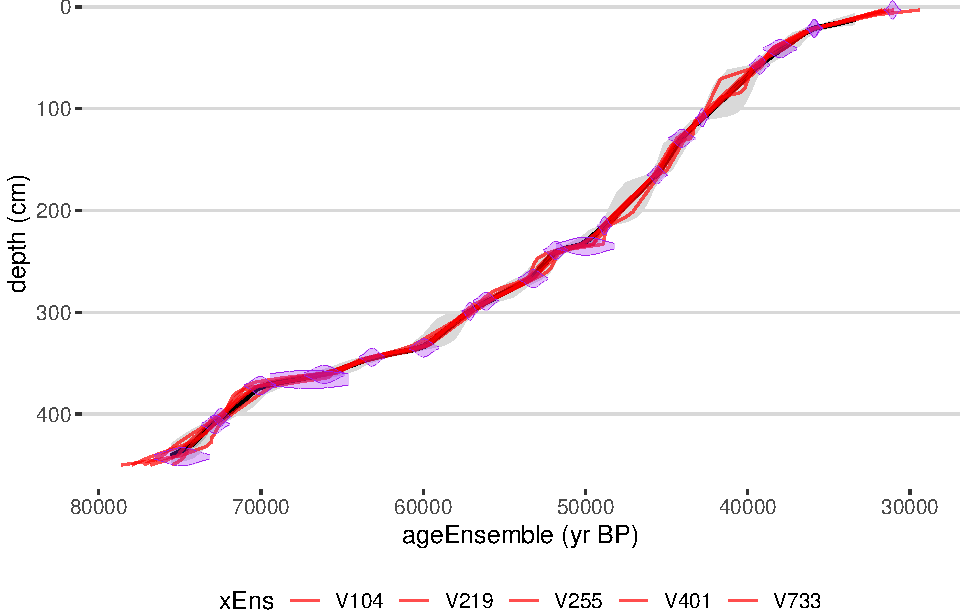
\includegraphics{geoChronR-paper_files/figure-latex/unnamed-chunk-3-1.pdf}
After an age ensemble has been added to a LiPD object, the user can
visualize the ensemble timeseries using
\texttt{plotTimeseriesEnsRibbons()} and
\texttt{plotTimeseriesEnsLines()}. GISP2 \(\delta^{18}\)O is plotted
with age uncertainty, using both functions, in figure x.

\begin{verbatim}
## Scale for 'x' is already present. Adding another scale for 'x', which will
## replace the existing scale.
\end{verbatim}

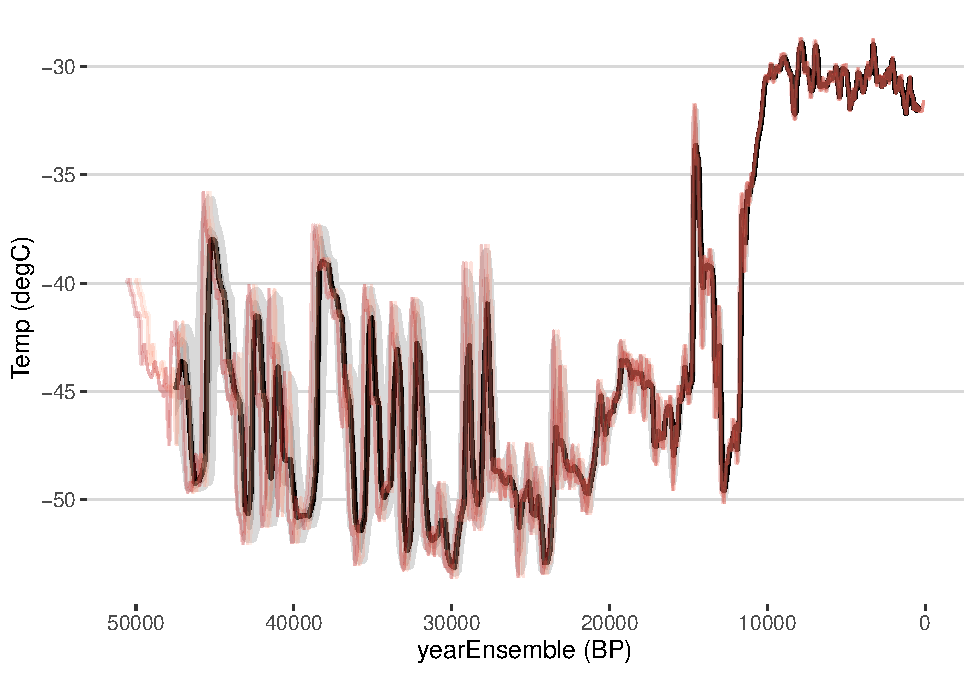
\includegraphics{geoChronR-paper_files/figure-latex/unnamed-chunk-5-1.pdf}

\subsection{Correlation}

Now that the user has generated age ensembles for the two datasets,
they're interested to see if a correlation between the two datasets is
robust to the age uncertainty modeled here. On multi-millennial
timescales, the two datasets have similarities, and previous work has
suggested that could events during the Last Glacial period, which are
observed in the GISP2 record, can impact the Asian Monsoon and be
observed is speleothem records such as the Hulu Cave dataset. (NM: add
references here and flesh out background) The \texttt{corEns()} function
in geoChronR will calculate ensemble correlations across age-uncertain
datasets, such as these. \texttt{corEns()} will also sample across
ensembles in the paleoData as well, if present. Here we calculate
correlations during the period of overlap in 500 yr steps, determining
significance for each pair of ensemble members while accounting for
autocorrelation.

The results show consistently negative correlations, although 13.45\% of
the ensemble members are positive. However, only 0.89\% are significant
after accounting for serial autocorrelation.

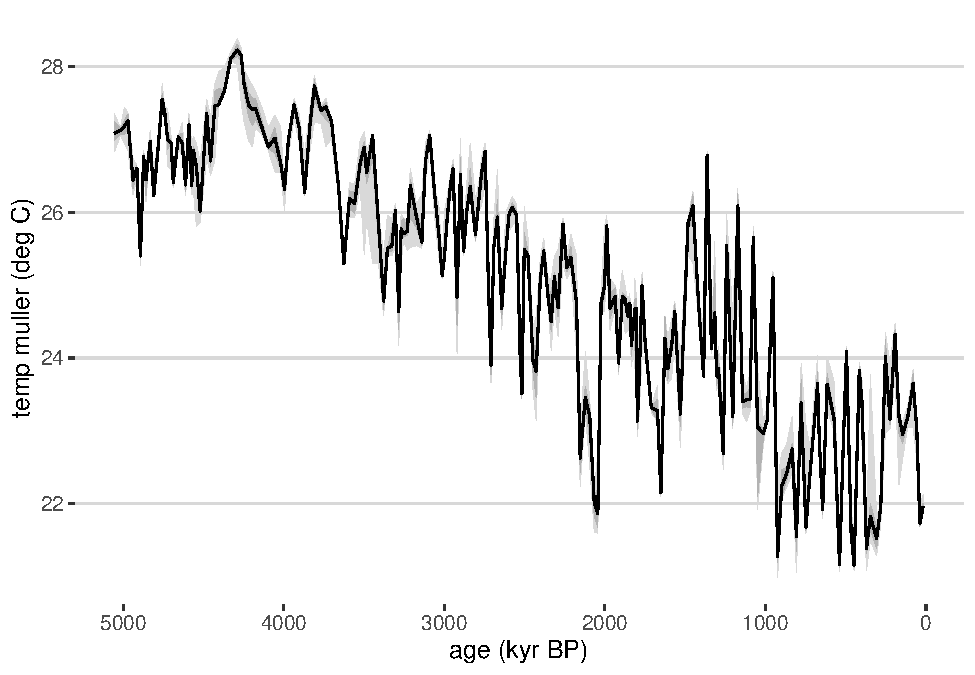
\includegraphics{geoChronR-paper_files/figure-latex/unnamed-chunk-7-1.pdf}
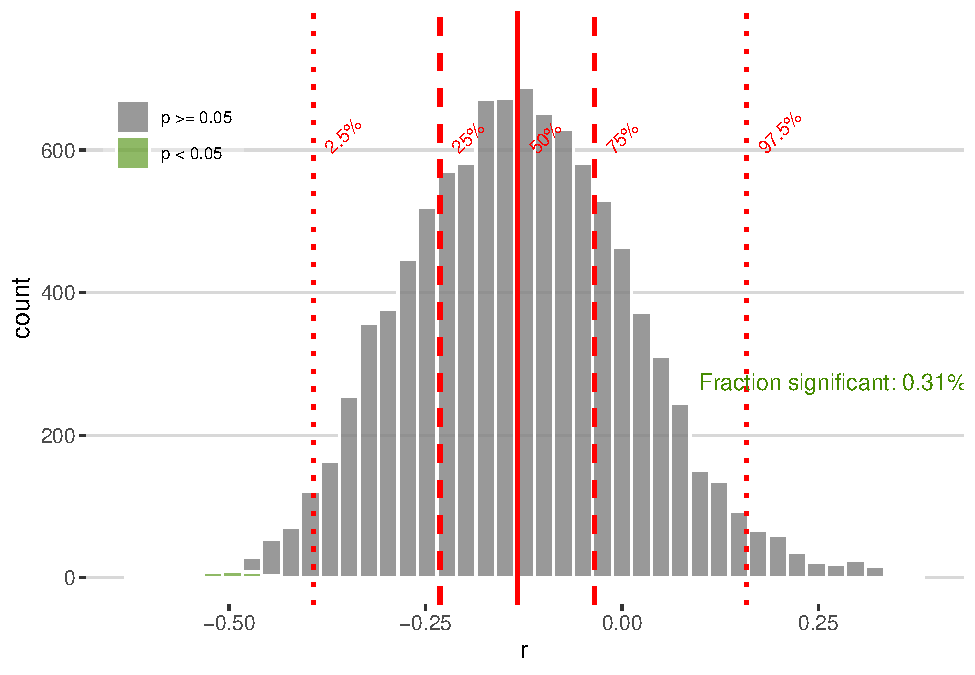
\includegraphics{geoChronR-paper_files/figure-latex/unnamed-chunk-7-2.pdf}

In this use case, we demonstrate how a user could calculate and
visualize and age-uncertain correlation between the Hulu speleothem d18O
record and the GISP2 ice core record. (Introduction about why a user
might want to do an age uncertain correlation between Hulu and GISP2).

\subsection{Regression}

A natural extension of ensemble correlation is ensemble regression.
Although there are use cases where regressing one age-uncertain variable
onto another is called for, here we regress an age-uncertain
paleoclimate proxy onto time-certain instrumental to develop a
calibration-in-time. For this use case, we reproduce the results of
\citet{Boldt:2015}, where the authors calibrate a spectral reflectance
measure of chlorophyll abundance to temperature in Northern Alaska.

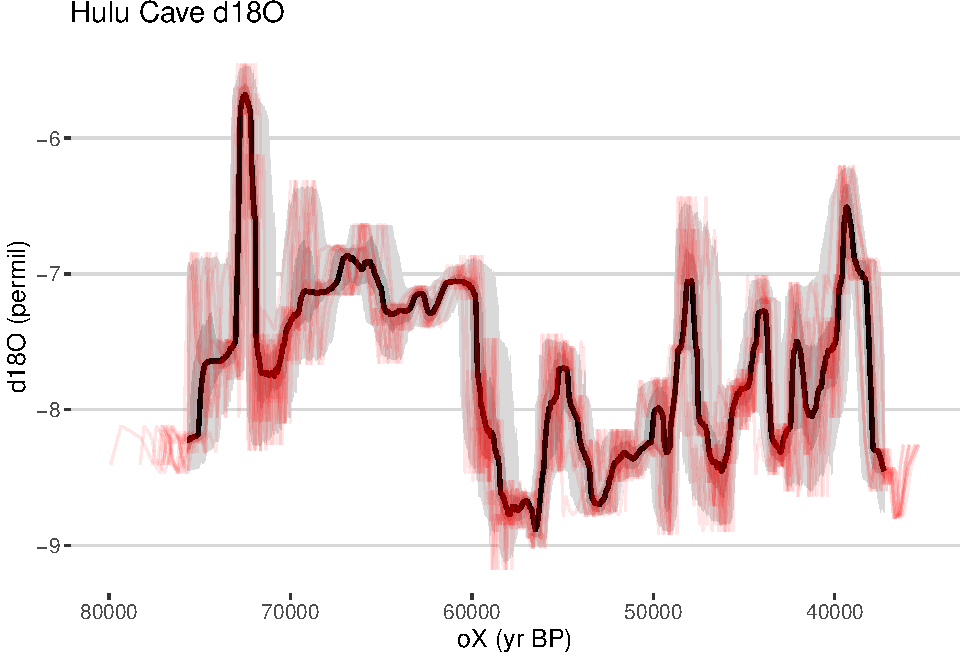
\includegraphics{geoChronR-paper_files/figure-latex/unnamed-chunk-9-1.pdf}
Figure captions.

\subsection{Principle Components Analysis}

\subsection{Spectral Analysis}

\section{Discussion \& Conclusion}

\begin{itemize}
\item
  Strengths, weaknesses and shortcomings of our approach
\item
  Next steps; where does age-uncertain work go from here?
\item
  GeoChronR plans, longevity, etc
\end{itemize}

\section{Everything below are useful examples of how to use RMarkdown}

Subsection text here.

\subsubsection{Subsubsection Heading Here}

Subsubsection text here.

\section{Content section with citations}

See the
\href{http://rmarkdown.rstudio.com/authoring_bibliographies_and_citations.html}{R
Markdown docs for bibliographies and citations}.

Copernicus supports biblatex. I put the .bib entries from the Paleocube
proposal into \texttt{geochronr.bib}. Citations work like this:

Read \citep{Evans_QSR13}, and \citep[see][]{PRYSM}.

\section{Content section with R code chunks}

You should always use \texttt{echo\ =\ FALSE} on R Markdown code blocks
as they add formatting and styling not desired by Copernicus. The hidden
workflow results in 42.

You can add verbatim code snippets without extra styles by using
\texttt{\textasciigrave{}\textasciigrave{}\textasciigrave{}} without
additional instructions.

\begin{verbatim}
sum <- 1 + 41
\end{verbatim}

\section{Content section with list}

If you want to insert a list, you must

\begin{itemize}
\item
  leave
\item
  empty lines
\item
  between each list item
\end{itemize}

because the \texttt{\textbackslash{}tightlist} format used by R Markdown
is not supported in the Copernicus template. Example:

\begin{verbatim}
- leave

- empty lines

- between each list item
\end{verbatim}

\section{Examples from the official template}

\subsection{FIGURES}

When figures and tables are placed at the end of the MS (article in
one-column style), please add \clearpage between bibliography and first
table and/or figure as well as between each table and/or figure.

\subsubsection{ONE-COLUMN FIGURES}

Include a 12cm width figure of Nikolaus Copernicus from
\href{https://en.wikipedia.org/wiki/File:Nikolaus_Kopernikus.jpg}{Wikipedia}
with caption using R Markdown.

\begin{figure}
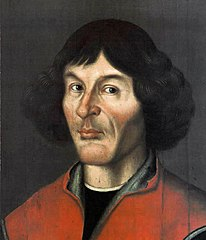
\includegraphics[width=8.3cm]{Nikolaus_Kopernikus} \caption{one column figure}\label{fig:unnamed-chunk-11}
\end{figure}

\subsubsection{TWO-COLUMN FIGURES}

You can also include a larger figure.

\begin{figure}
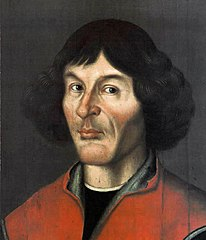
\includegraphics[width=12cm]{Nikolaus_Kopernikus} \caption{two column figure}\label{fig:unnamed-chunk-12}
\end{figure}

\subsection{TABLES}

You can ad \LaTeX table in an R Markdown document to meet the template
requirements.

\subsubsection{ONE-COLUMN TABLE}

\begin{table}[t]
\caption{TEXT}
\begin{tabular}{l c r}
\tophline

a & b & c \\
\middlehline
1 & 2 & 3 \\

\bottomhline
\end{tabular}
\belowtable{Table Footnotes}
\end{table}

\subsubsection{TWO-COLUMN TABLE}

\begin{table*}[t]
\caption{TEXT}
\begin{tabular}{l c r}
\tophline

a & b & c \\
\middlehline
1 & 2 & 3 \\

\bottomhline
\end{tabular}
\belowtable{Table footnotes}
\end{table*}

\subsection{MATHEMATICAL EXPRESSIONS}

All papers typeset by Copernicus Publications follow the math
typesetting regulations given by the IUPAC Green Book (IUPAC:
Quantities, Units and Symbols in Physical Chemistry, 2nd Edn., Blackwell
Science, available at:
http://old.iupac.org/publications/books/gbook/green\_book\_2ed.pdf,
1993).

Physical quantities/variables are typeset in italic font (t for time, T
for Temperature)

Indices which are not defined are typeset in italic font (x, y, z, a, b,
c)

Items/objects which are defined are typeset in roman font (Car A, Car B)

Descriptions/specifications which are defined by itself are typeset in
roman font (abs, rel, ref, tot, net, ice)

Abbreviations from 2 letters are typeset in roman font (RH, LAI)

Vectors are identified in bold italic font using \vec{x}

Matrices are identified in bold roman font

Multiplication signs are typeset using the LaTeX commands
\texttt{\textbackslash{}times} (for vector products, grids, and
exponential notations) or \texttt{\textbackslash{}cdot}

The character * should not be applied as mutliplication sign

\subsection{EQUATIONS}

\subsubsection{Single-row equation}

Unnumbered equations (i.e.~using \texttt{\$\$} and getting inline
preview in RStudio) are not supported by Copernicus.

\begin{equation}
1 \times 1 \cdot 1 = 42
\end{equation}

\begin{equation}
A = \pi r^2
\end{equation}

\begin{equation}
x=\frac{2b\pm\sqrt{b^{2}-4ac}}{2c}.  
\end{equation}

\subsubsection{Multiline equation}

\begin{align}
& 3 + 5 = 8\\
& 3 + 5 = 8\\
& 3 + 5 = 8
\end{align}

\subsection{MATRICES}

\[
\begin{matrix}
x & y & z\\
x & y & z\\
x & y & z\\
\end{matrix}
\]

\subsection{ALGORITHM}

If you want to use algorithms, you can either enable the required
packages in the header (the default, see \texttt{algorithms:\ true}), or
make sure yourself that the \LaTeX packages \texttt{algorithms} and
\texttt{algorithmicx} are installed so that \texttt{algorithm.sty}
respectively \texttt{algorithmic.sty} can be loaded by the Copernicus
template. Copernicus staff will remove all undesirable packages from
your LaTeX source code, so please stick to using the header option,
which only adds the two acceptable packages.

\begin{algorithm}
\caption{Algorithm Caption}
\label{a1}
\begin{algorithmic}
\STATE $i\gets 10$
\IF {$i\geq 5$} 
        \STATE $i\gets i-1$
\ELSE
        \IF {$i\leq 3$}
                \STATE $i\gets i+2$
        \ENDIF
\ENDIF
\end{algorithmic}
\end{algorithm}

\subsection{CHEMICAL FORMULAS AND REACTIONS}

For formulas embedded in the text, please use
\texttt{\textbackslash{}chem\{\}}, e.g. \chem{A \rightarrow B}.

The reaction environment creates labels including the letter R, i.e.
(R1), (R2), etc.

\begin{itemize}
\item
  \texttt{\textbackslash{}rightarrow} should be used for normal
  (one-way) chemical reactions
\item
  \texttt{\textbackslash{}rightleftharpoons} should be used for
  equilibria
\item
  \texttt{\textbackslash{}leftrightarrow} should be used for resonance
  structures
\end{itemize}

\begin{reaction}
A \rightarrow B \\
\end{reaction}
\begin{reaction}
Coper \rightleftharpoons nicus \\
\end{reaction}
\begin{reaction}
Publi \leftrightarrow cations
\end{reaction}

\subsection{PHYSICAL UNITS}

Please use \texttt{\textbackslash{}unit\{\}} (allows to save the
math/\texttt{\$} environment) and apply the exponential notation, for
example \(3.14\,\unit{km\,h^{-1}}\) (using LaTeX mode:
\texttt{\textbackslash{}(\ 3.14\textbackslash{},\textbackslash{}unit\{...\}\ \textbackslash{})})
or \unit{0.872\,m\,s^{-1}} (using only
\texttt{\textbackslash{}unit\{0.872\textbackslash{},m\textbackslash{},s\^{}\{-1\}\}}).

\conclusions

The conclusion goes here. You can modify the section name with
\texttt{\textbackslash{}conclusions{[}modified\ heading\ if\ necessary{]}}.




\codedataavailability{use this to add a statement when having data sets and software code
available} %% use this section when having data sets and software code available



%%%%%%%%%%%%%%%%%%%%%%%%%%%%%%%%%%%%%%%%%%
%% optional

%%%%%%%%%%%%%%%%%%%%%%%%%%%%%%%%%%%%%%%%%%
\appendix
\section{Figures and tables in appendices}

Regarding figures and tables in appendices, the following two options
are possible depending on your general handling of figures and tables in
the manuscript environment:

\subsection{Option 1}

If you sorted all figures and tables into the sections of the text,
please also sort the appendix figures and appendix tables into the
respective appendix sections. They will be correctly named
automatically.

\subsection{Option 2}

If you put all figures after the reference list, please insert appendix
tables and figures after the normal tables and figures.

To rename them correctly to A1, A2, etc., please add the following
commands in front of them: \texttt{\textbackslash{}appendixfigures}
needs to be added in front of appendix figures
\texttt{\textbackslash{}appendixtables} needs to be added in front of
appendix tables

Please add \texttt{\textbackslash{}clearpage} between each table and/or
figure. Further guidelines on figures and tables can be found below.
\noappendix

%%%%%%%%%%%%%%%%%%%%%%%%%%%%%%%%%%%%%%%%%%

%%%%%%%%%%%%%%%%%%%%%%%%%%%%%%%%%%%%%%%%%%
\competinginterests{The authors declare no competing interests.} %% this section is mandatory even if you declare that no competing interests are present

%%%%%%%%%%%%%%%%%%%%%%%%%%%%%%%%%%%%%%%%%%
\disclaimer{disc} %% optional section

%%%%%%%%%%%%%%%%%%%%%%%%%%%%%%%%%%%%%%%%%%
\begin{acknowledgements}
ack
\end{acknowledgements}

%% REFERENCES
%% DN: pre-configured to BibTeX for rticles

%% The reference list is compiled as follows:
%%
%% \begin{thebibliography}{}
%%
%% \bibitem[AUTHOR(YEAR)]{LABEL1}
%% REFERENCE 1
%%
%% \bibitem[AUTHOR(YEAR)]{LABEL2}
%% REFERENCE 2
%%
%% \end{thebibliography}

%% Since the Copernicus LaTeX package includes the BibTeX style file copernicus.bst,
%% authors experienced with BibTeX only have to include the following two lines:
%%
\bibliographystyle{copernicus}
\bibliography{geochronr.bib}
%%
%% URLs and DOIs can be entered in your BibTeX file as:
%%
%% URL = {http://www.xyz.org/~jones/idx_g.htm}
%% DOI = {10.5194/xyz}


%% LITERATURE CITATIONS
%%
%% command                        & example result
%% \citet{jones90}|               & Jones et al. (1990)
%% \citep{jones90}|               & (Jones et al., 1990)
%% \citep{jones90,jones93}|       & (Jones et al., 1990, 1993)
%% \citep[p.~32]{jones90}|        & (Jones et al., 1990, p.~32)
%% \citep[e.g.,][]{jones90}|      & (e.g., Jones et al., 1990)
%% \citep[e.g.,][p.~32]{jones90}| & (e.g., Jones et al., 1990, p.~32)
%% \citeauthor{jones90}|          & Jones et al.
%% \citeyear{jones90}|            & 1990

\end{document}
